\documentclass[10pt, a4paper, notitlepage, DIV=15]{scrartcl}
\usepackage[ngerman, english]{babel}
\usepackage[utf8]{inputenc}
\usepackage[T1]{fontenc}
\usepackage{csquotes}
\usepackage{xcolor}
\usepackage{amsmath}
\usepackage{amsfonts}
\usepackage{graphicx}
\usepackage{siunitx}
\usepackage{csquotes}
\usepackage{hyperref}
\usepackage[section]{placeins}

\title{Properties of Elementary Particles}
\author{Max Bock \\ Email \href{mailto:s6mabock@uni-bonn.de}{s6mabock@uni-bonn.de} 
	\and Marvin Hoffmann \\ Email \href{mailto:marvin.hoffmann@uni-bonn.de}{marvin.hoffmann@uni-bonn.de} }

%Nature has always looked like a horrible mess, but as we go along we see patterns and put theories together; a certain clarity comes and things get simpler. (Richard P. Feynman (R.P Feynam: QED- The Strange Theory of Light and Matter (Princeton UNiversity Press, Princeton 1985)))%


\begin{document}
\maketitle
\begin{abstract}
	\Large
	Nature has always looked like a horrible mess, but as we go along we see patterns and put theories together; a certain clarity comes and things get simpler. - Richard P. Feynman \cite{feynman}
\end{abstract}
\tableofcontents
\newpage

\section{Introduction}
In this experiment typical interactions in elementary particle physics will studied. Therefore, first proton-proton interactions observed in a bubble chamber are analysed. Further, the films from the bumble chamber are used to study $\pi$-$\mu$-e decays and observe strange neutral particles which have to be identified. In the end certain characteristics of $\omega$ mesons are determined in a computer-based analysis of many $\text{pp}\rightarrow\text{pp}\pi^+\pi^-\pi^0$ events.
\section{Theoretical Background}
\subsection{Basics of particle physics}
\subsubsection{Basics of Standard Model of Particle Physics}
The Standard Model of particle physics implies the unified theory of the electromagnetic, weak and strong interaction and decides the elementary particles into two classes, namely bosons and fermions. \newline
The bosons acts as exchange particles of the fundamental forces and have an integer spin. These ones are often called gauge bosons. There are eight massless gluons, which carry the colour charge of the strong force. Due to the fact that the gluons themselves have a colour charge, they interact with each other. The interaction range of the gluon is the smallest of all gauge bosons and is in the order of $1\,$fm. The massless photon is the exchange particle of the electromagnetic force, which has no electromagnetic charge. The range of this gauge boson is infinity. For the weak interaction there are two exchange particles, the $Z$ boson which carries no electromagnetic charge, whereby the $W^{\pm}$ bosons have a charge of $\pm 1$. The last boson is the so called Higgs particle- This is a scalar boson which delivers the mass of all particles which are coupled to the Higgs field.  \newline
The fermions are divided into two subclasses, the quarks and the leptons which are also subdivided into three generations. Each fermion has a corresponding anti particle with the same mass but opposite charge, including electric, weak and strong charge.\newline
The quarks are the only particles which interact strongly and carry colour charge but also interacts electromagnetic and weak. Due to the fact that the quarks can not appear alone apart they must form colour neutral formations. These formations are called hadrons which are divided into two classes, the mesons and the baryons. The mesons consist of a quark-antiquark pair and the baryons consist of three quarks. Each quark has either a charge of $2/3$ or $-1/3$ and further a spin of $1/2$. 
\newline
The leptons consist of electron, muon and tau with the corresponding neutrino. Whereas the neutrinos have no charge and only interacts weakly, the electron, muon and tau have a charge of $-1$ and interacts weakly and electromagnetically. Additionally, all leptons have a spin of $1/2$. Due to the fact that the muon and the tau have a higher mass than the electron, free muons and taus will decay most likely into an electron and further neutrinos in the last stable decay step, whereas the electron is stable. \cite{povh}
\begin{figure}[h]
	\centering
	\includegraphics[width=0.6\textwidth]{Standard_model.png}
	\caption{Standard Model of Elementary Particles.}
	\label{fig:standard_model}
\end{figure}
\FloatBarrier
\subsubsection{Relativistic Kinematics}
The ratio between moving mass $m$ and energy $E$ in relativistic kinematics is given by Einsteins famous equation \cite{rebhan}
\begin{equation}
	E=mc^2
\end{equation}
where $c$ is the speed of light. This equation can also be written as \cite{rebhan}
\begin{equation}
	E^2c^4=m_0^2c^4+\vec{p}\,^2c^2
\end{equation}
with the momentum vector $\vec{p}$ and the rest mass $m_0$, which is directly related to the mass $m$ via \cite{rebhan}
\begin{equation}
	m =\gamma m_0
\end{equation}
with the Lorentz factor $\gamma$ \cite{rebhan}
\begin{equation}
	\gamma = \frac{1}{\sqrt{1-\beta^2}} \quad \text{with} \quad \beta = \frac{v}{c} 
\end{equation}
If one defines the four-momentum $p$ as vector \cite{rebhan}
\begin{equation}
	p= \begin{pmatrix}
		E \\ \vec{p}
		\end{pmatrix}
\end{equation}
the invariant mass $M_n$ of a $n$-particle system will be given by \cite{rebhan}
\begin{equation}
	M_n^2 = \left( \sum p_i \right)^2 = \left( \sum E_i \right)^2 - \left( \sum \vec{p_i} \right)^2
\end{equation}
\subsection{Bubble Chamber}
Till the early 80's, the bubble chamber was one of the most popular devices for detecting high energy elementary particles at accelerators. Therefore, in  a chamber that can be seen in figure \ref*{fig:bubble-chamber} a liquid which is nearly below the critical boiling temperature gets sequentially decompressed and compressed by a piston. While the liquid is decompressed it reaches an overheated state in which ionizing particles cause bubbles along their tracks. A particle will be deflected by a magnetic field if the particle has a electric charge. These bubbles can be detected by the use of cameras at different angles.   
\begin{figure}[h]
	\centering
	\includegraphics[width=0.7\textwidth]{bubble-chamber}
	\caption{Illustration of a bubble chamber. \cite{wiki-bubble} - edited}
	\label{fig:bubble-chamber}
\end{figure}
\FloatBarrier
\subsection{Proton Proton interaction}
\subsubsection{Elastic and Inelastic Scattering}
In the elastic scattering the particles before and after the scattering process are identical. Further, the sum of kinetic energy and the momentum stay unchanged during the event. In the inelastic case the particles after the action must not be the same as before. In addition, the momentum is conserved but the kinetic energy is transferred into for instance binding or ionizing energy. \cite{povh}
\subsubsection{Cross-Section}
 The cross-section is one of the most important quantities for description and interpretation in scattering experiments. This is related to the quantum mechanically probability of a reaction between the incoming particle and the target. In a proton-proton interaction the cross-section $\sigma$ is given by \cite{description}
 \begin{equation}
 	\sigma=\frac{1}{nl}\ln\left(\frac{N_\text{p}}{N_\text{p}-N_i} \right) 
 \end{equation}
 with the concentration of scattering centres $n$, the observed length of the bubble chamber $l$, the number of incoming protons $N_\text{p}$ and the number of prime interactions between two protons $N_i$. \cite{martin}
\subsubsection{Radiation Length}
The radiation length is defined as the average range where the energy of an electron is reduced to $1/e$ by bremsstrahlung. Further, the mean free path of the e$^+$e$^-$ pair production process is approximately $7/9$ of the radiation length. The radiation length $X_0$ is given by \cite{thomson}
\begin{equation}
	X_0\approx\frac{1}{4\alpha n_n Z^2r_\text{e}^2\ln\left(287/Z^{1/2} \right) }
\end{equation}
where $n_n$ is the number density of nuclei, $r_\text{e}$ is the classical radius of an electron, $Z$ is the atomic number and the fine structure constant $\alpha$. \cite{thomson}
\subsection{$\omega$ Meson}
The $\omega$ meson is a vector meson ($J^P=1^-$) to which an isospin of $I=0$ can be assigned. The corresponding wave function can be written as \cite{povh}
\begin{equation}
	|\omega \rangle = \frac{1}{\sqrt{2}}\left\lbrace|u^\uparrow \bar{u}^\uparrow \rangle + |d^\uparrow \bar{d}^\uparrow \rangle\right\rbrace 
\end{equation}
\subsubsection{Breit-Wigner Distribution}
A resonance is a system of shortly lived bounded states which are formed by two partners in a collision. In this case, the mass dependence of the cross-section in the vicinity of the resonance mass of  $m_\omega$ is described by the Breit-Wigner formula \cite{description}
\begin{equation}
	\sigma_{BW}(m)=  \frac{\Gamma_\omega}{2\pi}\frac{1}{(m-m_\omega)^2+\Gamma_\omega^2/4}
\end{equation}
\subsubsection{Gauss Distribution}
The Gauss distribution is a good approximation to describe many phenomena in physics. The continuous distribution is given by \cite{gauss}
\begin{equation}
	\sigma_G(m)=\frac{1}{s\sqrt{2\pi}}e^{-\frac{1}{2}\left( \frac{m-m_\omega}{s}\right)^2} 
\end{equation} 
whereupon $s$ is the standard deviation. 
\subsubsection{Dalitz Plots}
To classify decays of three particles with the same mass Dalitz plots are often used to determine the spin and parity of resonances. Therefore the kinetic energies of the three particles $T_1$, $T_2$ and $T_3$ are presented in a two dimensional equilateral triangle diagram with three axes as shown in figure \ref{fig:dalitz}.
\begin{figure}[h]
	\centering
	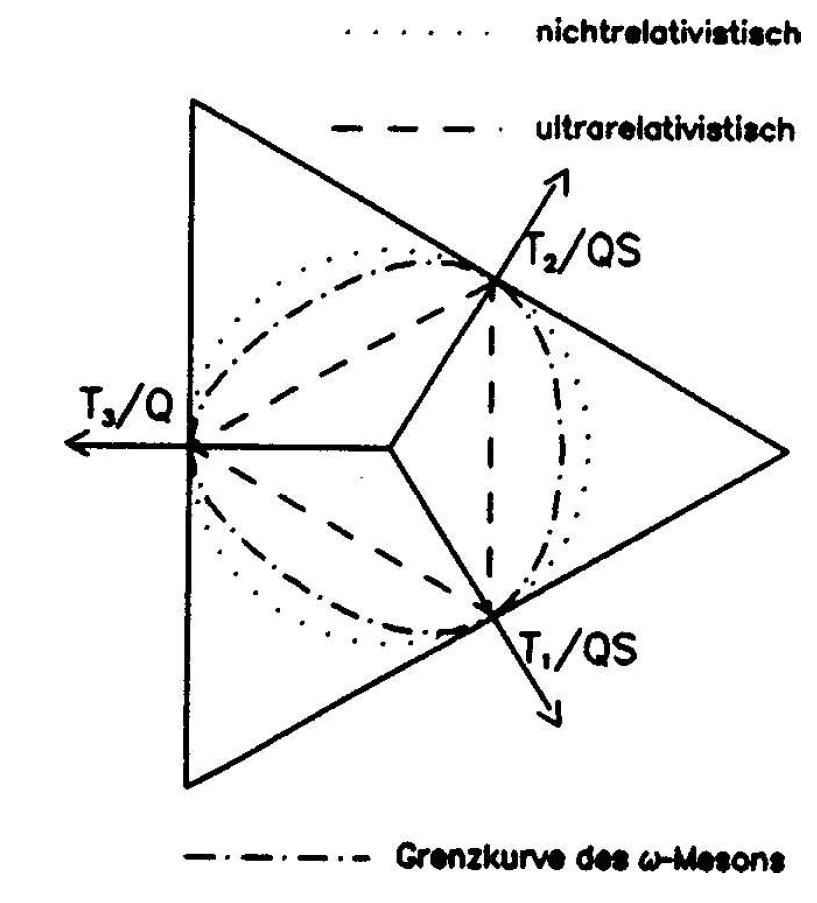
\includegraphics[width=0.6\textwidth]{Dalitz-triangle}
	\caption{Illustration of the Dalitz triangle. \cite{description}}
	\label{fig:dalitz}
\end{figure}
Each axis corresponds to the kinetic energy of one particle. Due to momentum conservation not every point in this triangle can be reached. In the non-relativistic case a perfect circle describes the reachable points whereas in the ultra-relativistic case this is described by an equilateral triangle. Each spin parity constellation is represented by different theoretical density distributions which is shown in figure \ref{fig:density_theo}.
\begin{figure}[h]
	\centering
	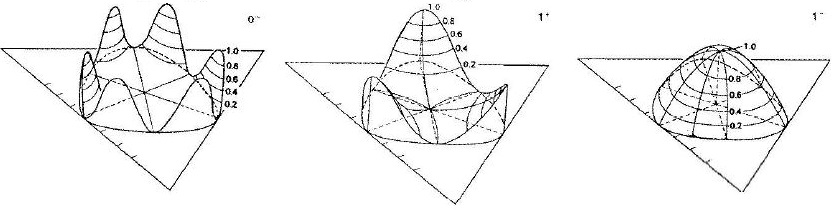
\includegraphics[width=1\textwidth]{density_theo}
	\caption{Density distribution for $J^P=0^-, 1^+ \,\text{and}\, 1^-$. \cite{description} - edited}
	\label{fig:density_theo}
\end{figure}

\section{Experimental Set-Up and Measurements}

\section{Analysis}
\subsection{Properties of proton-proton interaction using $24\,$GeV/c proton beam}
\subsubsection{Magnification}
\subsection{Weak decays}
\subsection{Determination of mass, lifetime, spin and parity of the $\omega$ meson}
\subsubsection{Bin Width}
First of all the best suitable bin width for the analysis has to be found. Therefore a Breit-Wigner distribution is fitted to the $\omega$ peak and for finding the most fitting bin width the reduced $\chi^2$ are compared. For that the fitting boarders are chosen between $600$ and $1100\,$MeV. This can be seen in table \textcolor{red}{!!!}. By this one can see that either a bin width of $11$ or $14$ are candidates for the best bin width. Due to the fact that the $\chi^2$ of the bin width of $11$ which is $1.0251$ is the best amount above the optimal value and the $\chi^2$ of the bin width of $14$ which is $0.985$ is the best amount below the optimal value $\chi^2=1$. Further these deviations are in the same order of magnitude. Due to that at this point of the analysis it is not possible to say which bin width is the optimal one. Therefore, a further observation is performed.
\subsubsection{Experimental Resolution}
For the experimental resolution a Gaussian function is fitted to the $\eta$ resonance as mentioned before. Because there are candidates for the best bin width this measurement is done for both ones with different fitting borders to compare the $\chi^2$ for all these fits. The $\chi^2$ for the different bin width and different fitting borders are shown in table \textcolor{red}{!!!}. As it is seen in table [!!!] the best $\chi^2$ is given for 
\section{Conclusion}

\section{Appendix}

\begin{thebibliography}{}
\bibitem{feynman}
	R. P. Feynam: \textit{QED- The Strange Theory of Light and Matter} (Princeton University Press, 1985)
\bibitem{povh}
	B. Povh, K. Rith, C. Scholz, F. Zetsche, W. Rodejohann: \textit{Teilchen und Kerne - Eine Einführung in die physikalischen Konzepte} (Springer Spektrum, 2014) 9th. edition
\bibitem{rebhan}
	E. Rebhan: \textit{Theoretische Physik: Relativitätstheorie und Kosmologie} (Spektrum, 2012) 1st. edition
	\bibitem{wiki-bubble}
	\url{https://en.wikipedia.org/wiki/Bubble_chamber#/media/File:Bubble-chamber.svg}\newline (last downloaded at 7th. April 2017)
\bibitem{description}
	G. Seul: \textit{Praktikumsversuche zur Einführung in die Hochenergyphysik} (Bonn, 1977)
\bibitem{martin} 
	B. R. Martin: \textit{Nuclear and Particle Physics - An Introduction} (Wiley, 2009) 2nd. edition
\bibitem{thomson}
	M. Thomson: \textit{Modern Particle Physics} (Cambridge University Press, 2015) 3rd. edition
\bibitem{gauss}
	L. Fahrmeir, A. Hamerle, G. Tutz: \textit{Multivariate statistische Verfahren} (Walter de Gruyter, 1996) 2nd. edition
\end{thebibliography}
 
\end{document}